\documentclass[10pt,twocolumn,letterpaper]{article}
\usepackage[review]{cvpr}
\usepackage{graphicx}
\usepackage{booktabs}
\usepackage{amsmath,amssymb}
\usepackage{multirow}
\usepackage{xcolor}
\usepackage{url}
\usepackage{microtype}
\graphicspath{{figures/}}

\definecolor{cvprblue}{rgb}{0.21,0.49,0.74}
\usepackage[pagebackref,breaklinks,colorlinks,allcolors=cvprblue]{hyperref}
\def\paperID{*****}
\def\confName{CVPR}
\def\confYear{2026}
\title{Measurement Count Is Not Influence:\
When Disagreement Hides MRI Interpolation Error}
\begin{document}
\maketitle

\begin{abstract}
Output disagreement can hide reconstruction error when two estimates depend on the same influential measurements. We test whether integer measurement overlap is an adequate description of this dependence in deterministic MRI inter-slice interpolation. For frozen HAT and SwinIR models, \emph{neural shared influence} is the cosine between centered finite-difference responses to the same physical slice anchor. Across fastMRI brain T2, 115 IXI brain T2 examinations, and patient-clustered NingXia knee T2, influence associates with error alignment, shared error fraction, and observable fraction more strongly than overlap count in all six dataset--architecture strata; 18 primary absolute-correlation advantages are 0.036--0.089 with clustered intervals above zero. With overlap fixed at one, the prediction holds on fastMRI/IXI but is mixed on NingXia. A prespecified stability audit passes all 42 amplitude/sign/field/direction strata (rank stability 0.942--0.999) but fails two of three physical-plane gates (0.779--0.954), bounding the statistic as local. Three preregistered method branches---context selection, multi-anchor jackknife, and covariance correction---also fail locked transfer/non-triviality gates. Thus reused measurements matter according to estimator response rather than count, but the result is a scoped mechanism finding, not a superior uncertainty estimator.
\end{abstract}

\section{Introduction}
Deterministic through-plane interpolation synthesizes missing MRI slices from sparse acquired anchors, but normally provides no indication of when a plausible image is wrong. Ensembles, test-time augmentation, and cross-context consistency convert output variation into reliability evidence \cite{lakshminarayanan2017ensembles,gal2016dropout,edupuganti2021uncertainty}. Their blind spot is common error: agreement observes $e_a-e_b$, not either reconstruction error itself.

We investigate how the measurement geometry of MRI interpolation governs this blindness. Our starting observation is that phase-shifted, measurement-disjoint contexts rank error better than contexts that reuse anchors. An exact analytical ladder had already falsified a tempting count-only law: the transition from zero to one shared anchor can be nonmonotone. But analytical coefficient weights do not establish what HAT or SwinIR actually use. We therefore define and evaluate a neural finite-difference influence quantity tied to common physical anchors. Across a broad context grid and a cleaner fixed-count subset, it tests whether continuous neural sensitivity explains error alignment beyond integer overlap.

The mechanism motivates a deployment-facing score audit. \emph{Acquired-anchor cross-validation} (Anchor-CV) withholds an interior acquired anchor, reconstructs it from adjacent anchors, and measures its residual. The operation is not new---leave-one-slice-out interpolation predates our work---and we freeze it before Plan6 evaluation. Its value, if any, must survive adjacent-anchor MAE/RMSE, scale, spacing, curvature, spectral, output-PC, and risk--coverage comparisons. We treat falsification of unique-information or superiority claims as part of the contribution.

Our contributions are: (1) a neural shared-influence response statistic evaluated on three cohorts and two architectures, with a prespecified perturbation/plane stability audit; (2) separate tests of influence$\rightarrow$alignment, alignment$\rightarrow$suppression, and influence$\rightarrow$observable fraction, with a heterogeneous final ranking arrow; and (3) a fixed-count falsification of integer overlap plus three failed method gates that delimit what the mechanism does not provide. Dense slices enter only retrospective evaluation; no result is presented as calibration, causal mediation, or a universally better reliability score.

\begin{figure*}[t]
\centering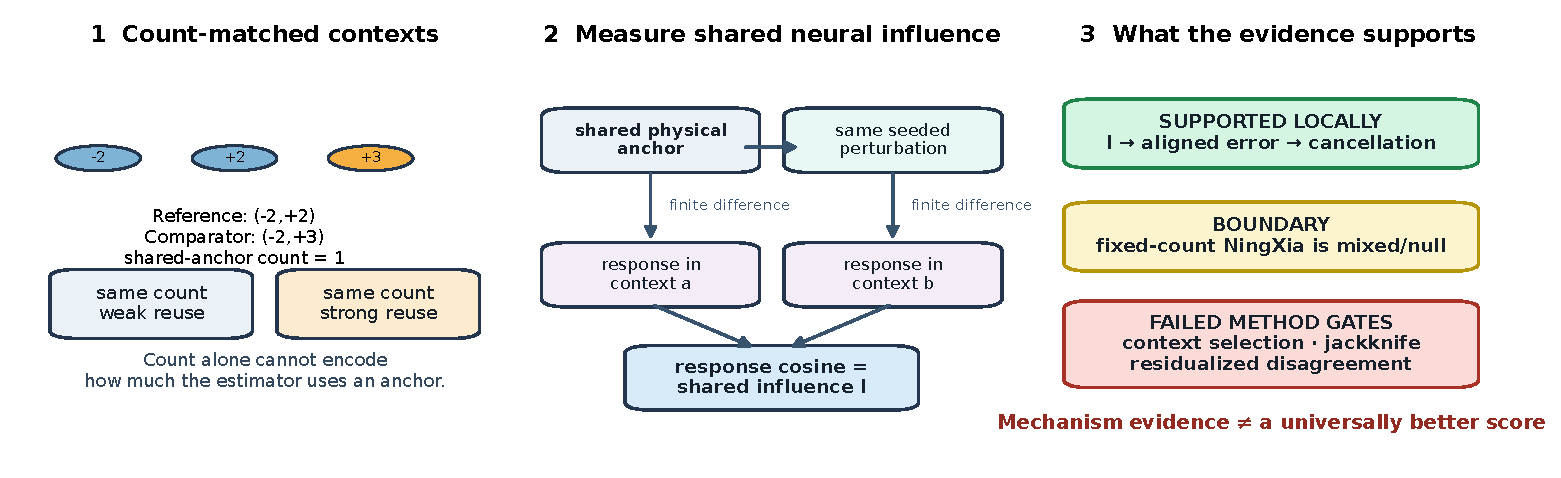
\includegraphics[width=.98\textwidth]{p7_fig1_mechanism_findings.pdf}
\caption{Count-matched contexts can reuse anchors with unequal estimator influence. We measure shared influence from paired finite-difference responses and test each mechanism arrow. Local associations are supported, NingXia limits universality, and three mechanism-derived reliability methods fail their locked gates.}
\label{fig:overview}
\end{figure*}

\section{Related Work}
\paragraph{Inter-slice MRI reconstruction.} SAINT introduced spatially aware medical slice synthesis \cite{peng2020saint}; I3Net combines inter- and intra-slice information \cite{song2024i3net}. Single-stack slice-to-volume reconstruction jointly treats motion and interpolation \cite{young2024svr}. Classical shifted multi-slice super-resolution acquires complementary measurements \cite{greenspan2002interslice}, while acquisition design has compared shifted and rotated schemes under Bayesian accuracy and precision \cite{nicastro2022shift}. These works improve reconstruction; we design reliability contexts for a frozen interpolator.

\paragraph{MRI uncertainty and active acquisition.} Learned MRI uncertainty includes variational/Bayesian reconstruction and deep ensembles \cite{narnhofer2022bayesian,kustner2024ensembles}. Active acquisition selects additional k-space measurements to reduce learned uncertainty \cite{zhang2019active}. Our setting is through-plane image-space interpolation. We neither learn a posterior nor optimize k-space: we study when output differences can observe error and derive a score from already acquired slice anchors.
Hu \etal showed that uncertainty variation can miss systematic MRI reconstruction error \cite{hu2021predict}; we therefore do not claim consensus blindness itself as novel. Likewise, leave-one-slice-out evaluation was used for medical interpolation \cite{horvath2017highorder}. Our novelty audit retains the physical measurement-dependence intervention, local neural shared-influence approximation, and frozen deployment-oriented evaluation role---not the algebra or holdout operation.

\paragraph{Consistency and shared error.} Predictive diversity interacts with individual error rather than replacing it \cite{brown2005diversity,ortega2022diversity}. MRI self-consistency, such as SPIRiT, enforces compatibility among acquired measurements \cite{lustig2010spirit}. Our distinction is intervention-level: the physical measurements supporting the same missing target are explicitly controlled, and their estimator influence is related to target-error alignment.

\section{Disagreement Observability}
For target slice $y$ and deterministic predictions $f_a=y+e_a$, $f_b=y+e_b$,
\begin{equation}
\|f_a-f_b\|^2=\|e_a\|^2+\|e_b\|^2-2\langle e_a,e_b\rangle. \label{eq:diff}
\end{equation}
Writing $\bar e=(e_a+e_b)/2$ and $\delta=(e_a-e_b)/2$ gives the exact decomposition
\begin{equation}
\tfrac12(\|e_a\|^2+\|e_b\|^2)=\|\bar e\|^2+\|\delta\|^2. \label{eq:decomp}
\end{equation}
We call the normalized terms the shared and observable fractions. If $e_a=e_b\ne0$, disagreement is zero despite error; if $e_a=-e_b$, all paired error energy is observable. Thus diversity is not calibration, and low disagreement cannot certify correctness.

\subsection{Shared Measurement Influence}
Let a local estimator be linear in its physical measurements, $f=\sum_j c_j x_j$. Two contexts are embedded in the union of physical anchor positions, yielding coefficient vectors $c_a,c_b$ with zeros at unused positions. Raw overlap counts common nonzero positions but ignores their influence. We test three acquisition-only summaries: coefficient cosine, signed dot product, and common absolute mass
\begin{equation}
I_{\cap}(a,b)=\sum_j\min(|c_{a,j}|,|c_{b,j}|). \label{eq:influence}
\end{equation}
All are target-free geometry/estimator properties for a linear estimator. They motivate but do not define influence for a nonlinear neural network. Let $F_c(x)$ denote a frozen interpolator under context $c$. For physical anchor $j$ shared by contexts $a,b$, apply the same seeded centered Rademacher perturbation $\epsilon\xi_{js}$ at 1\% of the globally normalized case range. The centered finite-difference response is
\begin{equation}
r_{cjs}=F_c(x+\epsilon\xi_{js})-F_c(x).
\end{equation}
We average the response cosine $\langle r_{ajs},r_{bjs}\rangle/(\|r_{ajs}\|\|r_{bjs}\|)$ over shared anchors and four frozen seeds (6101--6104). This \emph{neural shared influence} is a local sensitivity approximation around the observed input. It is not a global attribution theorem and does not identify influence from unshared anchors.

This definition separates three concepts that an integer count conflates. Two contexts may reuse one weak or one influential anchor; both receive the same overlap count but yield different shared responses. Response cosine measures directional alignment, while common response mass retains magnitude. Agreement among alternatives is a robustness check. Finite differences were chosen because they directly perturb acquired intensities and can be applied identically to HAT and SwinIR; no heatmap-based qualitative selection was used.

\section{Methods}
\subsection{Cohorts and Reconstruction Outputs}
The manifest contains 24 held-out fastMRI brain T2 cases \cite{knoll2020fastmri}, 22 out-of-fold NingXia knee T2 series from eight patients, and 115 held-out IXI brain T2 cases \cite{ixi_dataset}. Frozen HAT and SwinIR x4 predictions are evaluated; fastMRI/NingXia also have x2 outputs for retrospective densification benefit. NingXia inference resamples patient prefixes with all subordinate series retained. Physical planes are matched with NIfTI affines. Dense targets synthesize retrospective anchors and evaluate errors but never enter a reliability score. Evaluation uses a fixed foreground mask. All scores are reduced to one value per examination before cohort-level ranking, preventing long volumes from dominating the endpoint.

\subsection{Clean Overlap Controls}
The neural zero-overlap condition reconstructs the same missing plane from phase-0 and phase-2 x4 lattices. The clean maximal-overlap context applies horizontal flip equivariance to identical anchors, preserving z order, distance, count, mask, and preprocessing. The primary endpoint is Spearman correlation between masked prediction disagreement and paired MAE, with 5,000 examination/patient-cluster bootstrap replicates.

For an exact ladder, four anchors have target-relative absolute distances $\{1,2,3,4\}$. A reference sign pattern $(+,-,+,-)$ is compared with every sign pattern sharing exactly $k\in\{0,1,2,3,4\}$ positions and retaining anchors on both sides. A distance-weighted local linear regression, weights $1/d$, predicts the same target. We average all valid sign configurations at each $k$; no favorable arrangement is selected. A wider $\{2,4,6,8\}$ ladder is a depth-limited replication.

For the neural experiment, one central eligible target defines a reference context with offsets $(-2,+2)$ and eight target-preserving comparators. Target, input count, model, mask, and preprocessing are fixed; overlap, span, asymmetry, and physical identity are recorded. A registered stage gate expanded to three planes per examination only after every cohort/architecture had the expected endpoint direction and at least two cohorts improved over count. Confirmation therefore covers 72 fastMRI, 345 IXI, and 66 NingXia model-specific planes per architecture. The grid is broad rather than perfectly distance matched, so partial rank analyses control span, asymmetry, and examination.

A cleaner subset retains the four comparator contexts with exactly one shared anchor. Integer overlap is then constant. Neural influence is tested after controlling span, asymmetry, and examination. This is the strongest test that influence contains information beyond count; failure in NingXia is retained rather than averaged away.

\subsection{Acquired-Anchor Cross-Validation}
Given acquired x4 anchors $x_0,x_4,x_8,\ldots$, each interior $x_{4j}$ is withheld and predicted linearly from $x_{4(j-1)}$ and $x_{4(j+1)}$. Anchor-CV is the median masked MAE between predicted and actually acquired withheld anchors. It is model-independent and available before any denser acquisition. We compare case ranking with adjacent-anchor RMSE, analytical x8 bipartition disagreement, and the extra-grid phase score. Full allocation curves use 10/20/30/50\% budgets and include PC, TTA, committee, maximal-shared, random expectation, and oracle where compatible.

The median aggregation is prespecified to tolerate isolated motion or boundary failures. Importantly, Anchor-CV does not feed the withheld residual into the reconstruction model and does not assert exchangeability of individual planes. It asks a narrower question: whether an examination's acquired through-plane signal is locally predictable at the native sparse spacing. Retrospective correlation with x4 error and x4-to-x2 improvement tests whether that examination-level property is useful for triage.

Plan6 freezes the original identity-foreground masked half-second-difference implementation as ANCHOR\_CV\_V1. We reproduced every stored score from the frozen formula (maximum absolute difference $5.68\times10^{-14}$ after matching float32 masks) before examining new outcomes. Strong baselines include adjacent-anchor MAE/RMSE/SSIM, gradient and frequency differences, robust intensity range, spacing, curvature, first-difference variability, and output PC. Partial rank association conditions on adjacent MAE, scale, and spacing; leave-one-cluster-out ridge tests whether feature stacking explains the dominant examination effect without in-sample tuning.

IXI $\times2$ evidence was generated only after freezing checkpoint, SHA-256, preprocessing, metric, and 10/20/30/50\% budgets. The 115-case run is definition matched but cross-estimator: benefit is mean HAT/SwinIR $\times4$ error minus I3Net $\times2$ error. It tests case-level retrospective consequence, not a same-model causal treatment effect.

\subsection{Statistics}
The independent units are 24 fastMRI examinations, 115 IXI examinations, and eight NingXia patients. Plane results are descriptive; uncertainty uses 5,000 clustered bootstrap replicates. Paired bootstrap intervals compare Anchor-CV Spearman to locked comparators. No cohort-specific score transform or favorable budget selection is used. All new experiments are exploratory but were registered in the local experiment registry before their outputs were computed.
The full mechanism chain is evaluated arrow by arrow. Influence-to-error-alignment and influence-to-observable-fraction partial ranks control examination, span, and asymmetry. Alignment-to-normalized-disagreement additionally conditions on influence. Context-level ranking correlates each context's mean alignment/influence with its disagreement--error Spearman; with few contexts this final arrow has lower power. We describe the chain as conditional association, never causal mediation. The supplement reports every architecture stratum, frozen protocol, risk curve, budget interval, and material negative result.

\section{Results}
\subsection{Clean Sharing Produces Blindness}
Zero overlap ranks error better than the clean maximal-overlap control in all cohorts: the Spearman differences are 0.092 (95\% CI 0.043--0.176) on fastMRI, 0.193 (0.111--0.371) on NingXia, and 0.095 (0.078--0.126) on IXI. Clean-max error cosine is 0.949, 0.995, and 0.968, leaving observable error fractions of only 2.61\%, 0.25\%, and 1.58\%. Under zero-derived fixed quartile thresholds, clean sharing increases high-error/low-disagreement prevalence by 27.1\%, 28.2\%, and 20.9\%, with every clustered interval above zero.

The original order-reversal control supports the complete covariance chain on NingXia and IXI: overlap raises covariance and shared fraction while lowering observable fraction, disagreement, and ranking. Several arrows reverse on fastMRI, confirming that reversal is confounded and motivating the clean control.

\begin{table*}[t]
\centering
\caption{Clean same-target overlap control. $\Delta\rho$ is zero-overlap minus clean-maximal-overlap error-ranking correlation. Observable fraction is the paired error energy exposed by prediction difference. Stable-wrong is the prevalence increase under zero-derived fixed quartile thresholds. Intervals are clustered at examination/patient level.}
\label{tab:clean}
\small
\setlength{\tabcolsep}{3pt}
\begin{tabular}{lcccc}
\toprule
Cohort & Independent units & $\Delta\rho$ [95\% CI] & Clean-max error cosine & Clean-max observable / stable-wrong $\Delta$ \\
\midrule
fastMRI brain T2 & 24 examinations & .092 [.043, .176] & .949 & 2.61\% / +27.1 pp \\
IXI brain T2 & 115 examinations & .095 [.078, .126] & .968 & 1.58\% / +20.9 pp \\
NingXia knee T2 & 8 patients (22 series) & .193 [.111, .371] & .995 & 0.25\% / +28.2 pp \\
\bottomrule
\end{tabular}
\end{table*}

\subsection{An Exact Ladder Falsifies the Count-Only Law}
Figure~\ref{fig:ladder} shows all compact ladder levels. Overall trends have the predicted signs in every cohort: overlap-count trend is $+0.9$ for error cosine/shared fraction, $-0.9$ for observable fraction, and $-0.9$ to $-1.0$ for disagreement. However, every cohort violates strict monotonicity at $0\rightarrow1$: one shared anchor slightly lowers error cosine and increases observable fraction. Reliability correlation remains 0.958--0.992 for every nonidentical level. The wide ladder replicates the exception in IXI while NingXia is strictly monotone. Therefore count is associated with the mechanism but is not its sufficient causal dose.

\begin{figure}[t]
\centering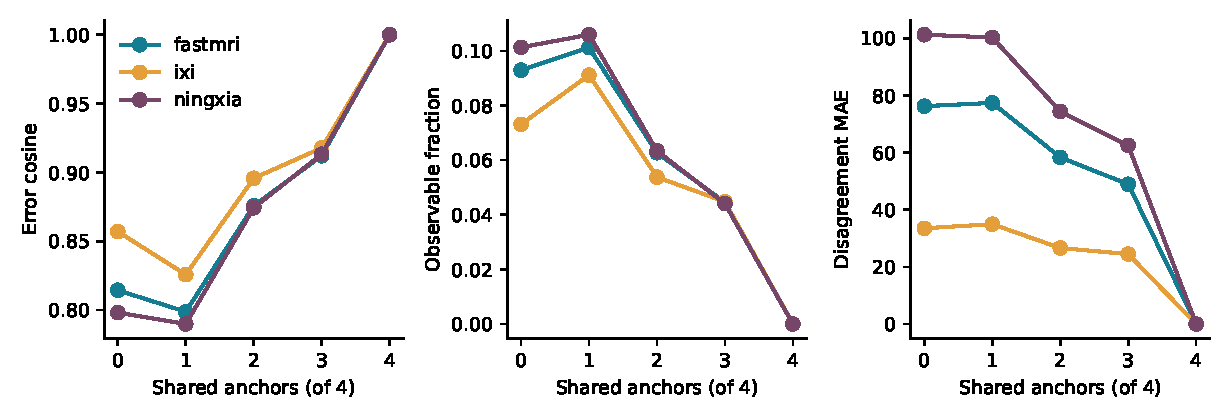
\includegraphics[width=\linewidth]{fig_compact_overlap_ladder.pdf}
\caption{Exact compact four-anchor ladder. Target, measurement count, absolute distances, estimator, and mask are fixed. Overall trends are strong, but the preserved $0\rightarrow1$ exception falsifies strict count monotonicity.}
\label{fig:ladder}
\end{figure}

\subsection{Neural Influence Explains More Than Count}
The registered stage gate passed, so the neural experiment expanded to three planes per examination. Figure~\ref{fig:neural} and Table~\ref{tab:neural} summarize the confirmatory endpoints. Neural influence had stronger absolute association than overlap count with error cosine, shared fraction, and observable fraction in all six dataset--architecture strata. The advantage was 0.036--0.089; all 18 examination/patient-cluster bootstrap intervals excluded zero. Rank-residual correlation of neural influence after overlap, span, asymmetry, and examination control remained $|\rho|=0.185$--0.395.

The result is not driven by one network. HAT/SwinIR influence-to-error-cosine correlations were 0.838/0.851 on fastMRI, 0.797/0.787 on IXI, and 0.786/0.772 on NingXia. Corresponding overlap-count correlations were 0.799/0.796, 0.714/0.712, and 0.743/0.735. Disagreement magnitude improved only modestly over count, and both fastMRI advantage intervals crossed zero. We therefore treat direct disagreement as supporting, not confirmatory, evidence.

\begin{figure}[t]
\centering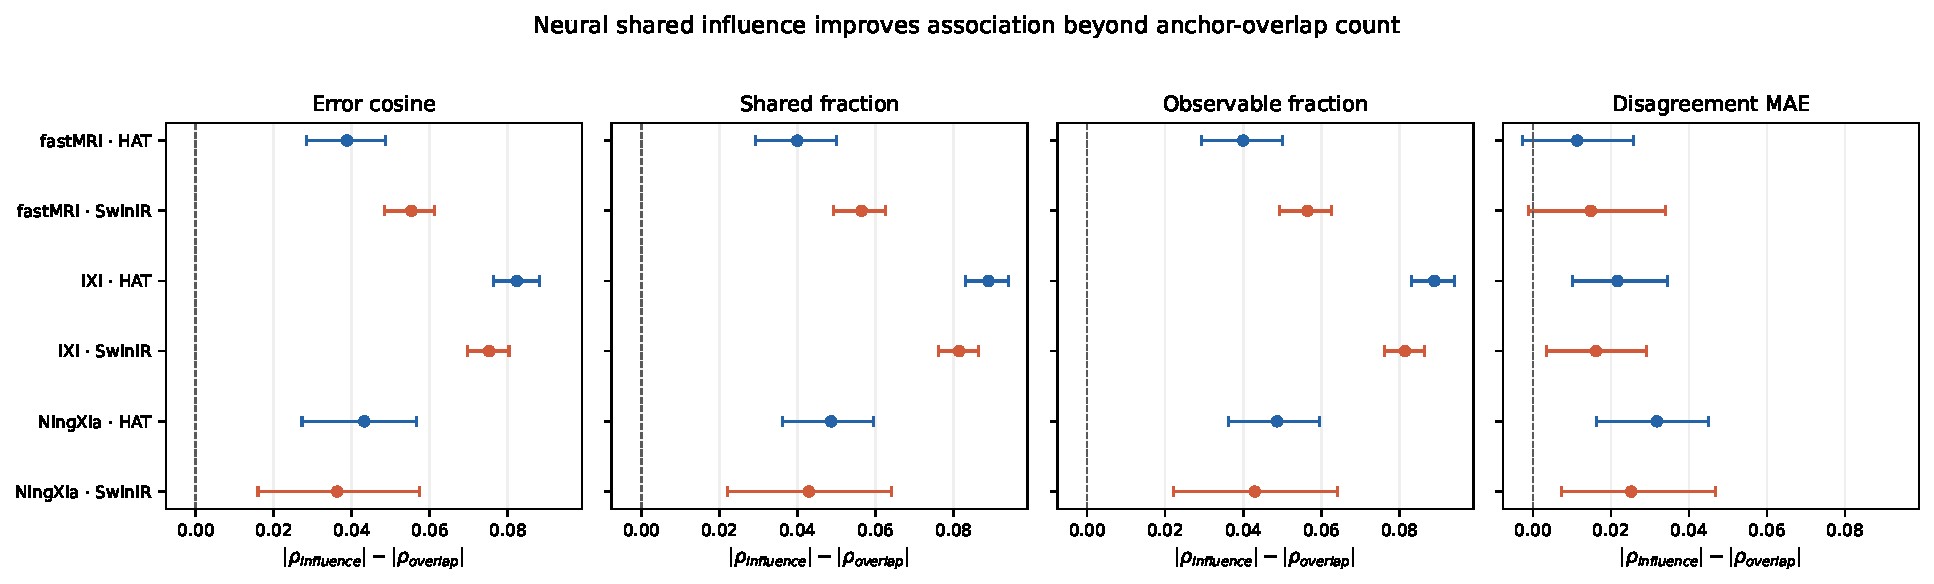
\includegraphics[width=\linewidth]{plan6_neural_influence_forest.pdf}
\caption{Neural finite-difference shared influence versus integer overlap. Forest intervals show the absolute-correlation advantage for error alignment, shared fraction, observable fraction, and supporting disagreement across frozen architectures/cohorts.}
\label{fig:neural}
\end{figure}

\begin{table}[t]
\centering
\caption{Influence versus overlap for error cosine}
\label{tab:neural}
\setlength{\tabcolsep}{3.5pt}
\begin{tabular}{llrrr}
\toprule
Cohort&Model&$\rho_{\rm count}$&$\rho_{\rm neural}$&Adv.\\
\midrule
fastMRI&HAT&.799&.838&.039\\
&SwinIR&.796&.851&.055\\
IXI&HAT&.714&.797&.082\\
&SwinIR&.712&.787&.075\\
NingXia&HAT&.743&.786&.043\\
&SwinIR&.735&.772&.036\\
\bottomrule
\end{tabular}
\end{table}

\subsection{Fixed-Count Test Rejects Universality}
Holding overlap exactly at one shared anchor removes count as an explanation. On fastMRI and IXI, neural influence retained the expected partial association with every endpoint/model after span, asymmetry, and examination control: $|\rho|=0.135$--0.587 and all clustered intervals excluded zero. For example, error-cosine partial $\rho$ was 0.169/0.350 on fastMRI HAT/SwinIR and 0.346/0.258 on IXI.

NingXia did not replicate the fixed-count result. Error-cosine partial $\rho$ was 0.014 for HAT and $-0.039$ for SwinIR; every endpoint interval crossed zero and several directions reversed. The broad-grid advantage in NingXia therefore does not establish continuous influence beyond count/geometry under eight-patient fixed-count inference. We reject a universal law and retain two supported claims: neural influence improves the broad descriptor in all cohorts, and beyond-count evidence is clean only in the two larger cohorts.

\begin{table*}[t]
\centering
\caption{Fixed-one-overlap neural influence partial Spearman after span, asymmetry, and examination control. Parentheses are clustered 95\% intervals for error cosine; $O$ is observable fraction and $D$ is disagreement.}
\label{tab:fixed}
\setlength{\tabcolsep}{4pt}
\begin{tabular}{llrrrr}
\toprule
Cohort&Model&Error cosine&Shared fraction&Observable $O$&Disagreement $D$\\
\midrule
fastMRI&HAT&.169 [.053,.283]&.135&$-.135$&$-.161$\\
&SwinIR&.350 [.212,.464]&.321&$-.321$&$-.286$\\
IXI&HAT&.346 [.259,.424]&.360&$-.360$&$-.543$\\
&SwinIR&.258 [.181,.335]&.241&$-.241$&$-.587$\\
NingXia&HAT&.014 [$-.232$,.223]&$-.006$&.006&$-.102$\\
&SwinIR&$-.039$ [$-.175$,.144]&$-.039$&.039&$-.072$\\
\bottomrule
\end{tabular}
\end{table*}

\subsection{The Local Chain Is Stronger Than the Ranking Chain}
The full mechanism was evaluated as four separate arrows. Influence associated with error alignment after examination and geometry control in all six strata ($\rho=0.219$--0.410); alignment associated with suppressed normalized disagreement conditional on influence/geometry ($\rho=-0.933$ to $-0.889$); and influence associated with lower observable fraction ($\rho=-0.412$ to $-0.211$). All 18 local-arrow intervals excluded zero.

The final context-level consequence was weaker. Greater alignment predicted poorer disagreement--error ranking in all strata, but intervals excluded zero only for both IXI models and NingXia HAT. Influence-to-ranking was less stable still. This asymmetry prevents a causal-mediation claim: finite-difference sensitivity explains local error geometry, while a small set of contexts and case mixtures determine whether that geometry changes a global ranking statistic.

\begin{table*}[t]
\centering
\caption{Mechanism-chain partial Spearman ranges across HAT/SwinIR. Every local-arrow interval excludes zero. Context-ranking support counts architecture strata whose interval excludes zero.}
\label{tab:chain}
\scriptsize
\setlength{\tabcolsep}{3.2pt}
\begin{tabular}{lrrrr}
\toprule
Cohort&Influence$\rightarrow$alignment&Alignment$\rightarrow$norm. disagreement&Influence$\rightarrow$observable&Alignment$\rightarrow$ranking\\
\midrule
fastMRI&.372--.410&$-.933$--$-.926$&$-.412$--$-.370$&$-.333$--$-.143$ (0/2 supported)\\
IXI&.321--.347&$-.893$--$-.890$&$-.342$--$-.298$&$-.643$--$-.500$ (2/2 supported)\\
NingXia&.219--.258&$-.898$--$-.889$&$-.231$--$-.211$&$-.667$--$-.548$ (1/2 supported)\\
\bottomrule
\end{tabular}
\end{table*}

The first and fourth arrows should not be conflated. A local context pair can have aligned errors because common influential anchors drive both outputs. Whether a \emph{set} of contexts then yields worse global case ranking depends on the distribution of error magnitude, target anatomy, and the finite number of context configurations. Strong local cancellation is necessary evidence for the proposed mechanism but is not sufficient for a universal context-level ranking theorem.

\subsection{The Mechanism Does Not Automatically Yield a Better Score}
We subjected four candidate capabilities to locked tests rather than selecting a favorable method after seeing transfer outcomes. First, frozen acquired-anchor cross-validation ranks x4 error strongly ($\rho=.943/.955/.958$ on fastMRI/IXI/NingXia), but adjacent MAE gives $.934/.956/.973$ and its conditional association beyond adjacent MAE, scale, and spacing is $.333/-.059/-.100$. The holdout operation predates this work and is retained only as a transparent negative audit.

Second, choosing the minimum-influence context among four fixed-count candidates performs well on 12 fastMRI confirmation cases ($\rho=.986/.965$ for HAT/SwinIR), but transfers below random-context expectation and output PC on IXI ($.973/.977$ versus random $.983/.983$ and PC $.994/.994$). NingXia is heterogeneous. Third, development-selected multi-anchor residual IQR collapses from $.629$ on fastMRI development to $.399$ on confirmation versus $.944$ for adjacent MAE; transfer correlations are $.732$ versus $.956$ on IXI and $.310$ versus $.973$ on NingXia. Fourth, the zero-fit covariance correction $d/\sqrt{1-I}$ ties or reduces raw disagreement on fastMRI confirmation, improves IXI by only $.0011/.0006$ with intervals crossing zero, and is mixed on NingXia. None passes the prespecified non-triviality/transfer gate (Table~\ref{tab:p7-gates}).

\begin{table*}[t]
\centering
\caption{Plan7 method gates. Development choices were frozen before confirmation/transfer; failure is not followed by test-cohort retuning.}
\label{tab:p7-gates}
\setlength{\tabcolsep}{4pt}
\begin{tabular}{p{3.2cm}p{3.4cm}p{5.4cm}p{2.0cm}}
\toprule
Candidate&Mechanistic rationale&Locked result&Decision\\
\midrule
Minimum-influence context&Expose error by reducing common response&Strong fastMRI confirmation; below random/PC on IXI; heterogeneous NingXia&Falsified\\
Multi-anchor jackknife IQR&Capture higher-order acquired difficulty&Confirmation/transfer far below adjacent MAE&Falsified\\
Influence residual $d/\sqrt{1-I}$&Undo predicted cancellation&Negligible IXI gain; tie/loss on fastMRI; mixed NingXia&Falsified\\
Anchor-CV V1&Use a measured pseudo-target&Strong rank, no consistent information beyond adjacent difference&Demoted\\
\bottomrule
\end{tabular}
\end{table*}

These failures do not negate the local mechanism: a descriptor can explain paired error geometry without producing an examination-level ranking rule. They do negate the stronger story that shared influence already creates a new deployment capability. Complete risk curves, densification budgets, efficiency, calibration, failure panels, and every unfavorable comparison remain in the supplement.

\section{Discussion}
The experiments refine a coarse observation into a neural mechanism with explicit limits. Measurement sharing aligns reconstruction errors and hides them from disagreement, but simply counting shared anchors is inadequate. Identically perturbing common physical anchors reveals how similarly each frozen network responds. This local neural influence improves explanation of error geometry over count in every broad-grid stratum and survives an exact fixed-count test in the two larger cohorts. It does not produce a validated superior score.

\paragraph{Why this is more than niche MRI.} The measured anchors are imaging-specific, but the distinction between shared information and shared output influence applies to any paired reliability estimator whose members reuse observations. Two predictors can have the same overlap count yet different local sensitivities, and a perturbation that changes appearance may preserve the relevant error direction. MRI makes the dependence physically auditable because anchor identity and target position are known. Generalization to other inverse problems is a hypothesis, not an evaluated claim.

\paragraph{Why finite differences.} Input gradients, integrated gradients, occlusion, and leave-one-anchor-out could all define sensitivity. Finite differences were selected before endpoint computation because they test the actual frozen input--output map, permit identical perturbations in two contexts, and avoid assuming differentiability through preprocessing. The Plan7 audit varies amplitude, sign/field, direction count, physical plane, cohort, and architecture under a prespecified rank-stability gate. All 42 perturbation-parameter strata pass (minimum $\rho=.942$), whereas only one of three plane-pair gates passes (minimum $\rho=.779$). The statistic is therefore a stable local probe at a declared plane, not a plane-invariant global Jacobian or attribution theorem.

Anchor-CV does not complete a ``mechanism produces a superior method'' story. It is cheap and strongly ranks examination difficulty and densification consequence, but adjacent difference explains nearly all of its rank information and output PC wins IXI benefit ranking. The three new Plan7 branches also fail transfer gates. These results prevent a method contribution from being inferred from a successful explanatory statistic.

The work does not estimate calibrated uncertainty, select a prospective scanner sequence, or establish clinical safety. Finite differences are local to the observed input, perturbation distribution, and amplitude; they do not identify a global neural Jacobian or causal mediation. Comparator contexts vary span/asymmetry, and the fixed-count NingXia result is null/mixed under only eight patients. IXI x2 is cross-estimator. A prospective policy should freeze the pilot, cost model, and threshold, then evaluate new acquisitions without dense-target leakage.

\paragraph{What the negative results change.} A strict ``less overlap is always better'' prescription is unsupported by the analytical $0\rightarrow1$ exception. A universal ``neural influence beyond count'' law is unsupported by fixed-count NingXia. Anchor-CV uniqueness, influence-aware context selection, multi-anchor dispersion, and covariance correction are falsified by adjacent MAE, output PC, random selection, or locked transfer. The remaining contribution is a scoped finding: continuous neural influence is a better broad context descriptor and locally supports alignment/cancellation, but no tested rule turns that explanation into a universally better reliability score.

\paragraph{Deployment interpretation.} Adjacent difference and Anchor-CV can be computed from an acquired sparse examination, while output PC requires stored model outputs and finite-difference influence requires extra neural evaluations. The present evidence supports retrospective ranking under fixed budgets, not autonomous reacquisition. Scanner time, motion risk, anatomy, and clinical urgency are absent from the utility function.

\paragraph{Patient-level inference.} NingXia contributes 22 series but only eight independent patients. Every clustered interval carries all series, models, planes, and contexts of a patient together. This produces wider and sometimes null fixed-count results despite hundreds of output comparisons. Treating series or planes as patients would have made the mechanism appear artificially universal. We retain NingXia as an informative heterogeneous boundary, not an equally powered confirmation cohort.

\paragraph{Efficiency and failure.} Anchor-CV takes 0.42/3.97/3.93 ms CPU on fastMRI/IXI/NingXia with zero neural calls, but adjacent difference is equally deployment-valid and often as accurate. Output PC is cheap only after two predictions exist; finite-difference influence is a research probe rather than the recommended QA score. Detailed timing and rare PC/Anchor discordance are supplementary because no fusion or superiority claim survived.

\paragraph{Reproducibility and scope.} Each claim is linked to a registered experiment, manifest, per-case/configuration output, and clustered summary. Finite-difference conditions, contexts, checkpoints and method gates were frozen. We report fixed-count NingXia heterogeneity, all three failed Plan7 methods, scale dependence, feature-stacking failure and failed localization. No local association is presented as a global theorem.

\section{Conclusion}
Disagreement reveals only error components that differ between reconstruction contexts. In MRI inter-slice interpolation, local neural shared influence describes error alignment and observable fraction more precisely than shared-anchor count across three broad context grids, with fixed-count confirmation limited to fastMRI and IXI. Yet context selection, multi-anchor jackknife, covariance correction, and acquired-anchor cross-validation do not outperform trivial baselines consistently. The supported message is mechanistic rather than prescriptive: measurement count is not estimator influence, and explaining why agreement hides error does not itself solve reliability ranking.

{\small
\bibliographystyle{ieeenat_fullname}
\bibliography{references}
}
\end{document}
